\documentclass[journal,12pt,onecolumn]{IEEEtran}
\usepackage{cite}
\usepackage{graphicx}
\usepackage{amsmath,amssymb,amsfonts,amsthm}
\usepackage{algorithmic}
\usepackage{graphicx}
\usepackage{textcomp}
\usepackage{xcolor}
\usepackage{txfonts}
\usepackage{listings}
\usepackage{enumitem}
\usepackage{mathtools}
\usepackage{gensymb}
\usepackage{comment}
\usepackage[breaklinks=true]{hyperref}
\usepackage{tkz-euclide} 
\usepackage{listings}
\usepackage{gvv}                                        
%\def\inputGnumericTable{}                                 
\usepackage[latin1]{inputenc}
\usetikzlibrary{arrows.meta, positioning}
\usepackage{xparse}
\usepackage{color}                                            
\usepackage{array}                                            
\usepackage{longtable}                                       
\usepackage{calc}                                             
\usepackage{multirow}
\usepackage{multicol}
\usepackage{hhline}                                           
\usepackage{ifthen}                                           
\usepackage{lscape}
\usepackage{tabularx}
\usepackage{array}
\usepackage{float}
\newtheorem{theorem}{Theorem}[section]
\newtheorem{problem}{Problem}
\newtheorem{proposition}{Proposition}[section]
\newtheorem{lemma}{Lemma}[section]
\newtheorem{corollary}[theorem]{Corollary}
\newtheorem{example}{Example}[section]
\newtheorem{definition}[problem]{Definition}
\newcommand{\BEQA}{\begin{eqnarray}}
\newcommand{\EEQA}{\end{eqnarray}}
\usepackage{float}
%\newcommand{\define}{\stackrel{\triangle}{=}}
\theoremstyle{remark}
\usepackage{circuitikz}
\usepackage{tikz}
\usepackage{ragged2e}

\begin{document}
\centering
\textbf{Environmental Science and Engineering\brak{\text{ES}}}
\begin{enumerate}
\item Rafi told Mary, "I am thinking of watching a film this weekend." 
The following reports on the above statement in indirect speech:\\ Rafi told Mary that 
\underline{\hspace{2cm}} of watching a film that weekend.
\begin{enumerate}
\begin{multicols}{4}
\item thought
\item is thinking
\item am thinking
\item was thinking
\end{multicols}
\end{enumerate}
\hfill{\brak{\text{GATE ES 2023}}}
\item Permit : \underline{\hspace{2cm}} :: Enforce : Relax \\
\brak{\text{By word meaning}}
\begin{enumerate}
\begin{multicols}{4}
\item Allow
\item Forbid
\item License
\item Reinforce
\end{multicols}
\end{enumerate}
\hfill{\brak{\text{GATE ES 2023}}}
\item Given a fair six-faced dice where the faces are labelled `1', `2', `3', `4', `5', and `6', what is the probability of getting a `1' on the first roll of the dice and a `4' on the second roll?
\begin{enumerate}
\begin{multicols}{4}
\item $\frac{1}{36}$
\item $\frac{1}{6}$
\item $\frac{5}{6}$
\item $\frac{1}{3}$
\end{multicols}
\end{enumerate}
\hfill{\brak{\text{GATE ES 2023}}}
\item A recent survey shows that $65\%$ of tobacco users were advised to stop consuming tobacco. 
The survey also shows that 3 out of 10 tobacco users attempted to stop using tobacco. \\
Based only on the information in the above passage, which one of the following options can be logically inferred with certainty?
\begin{enumerate}
\item A majority of tobacco users who were advised to stop consuming tobacco made an attempt to do so.
\item A majority of tobacco users who were advised to stop consuming tobacco did not attempt to do so.
\item Approximately $30\%$ of tobacco users successfully stopped consuming tobacco.
\item Approximately $65\%$ of tobacco users successfully stopped consuming tobacco.
\end{enumerate}
\hfill{\brak{\text{GATE ES 2023}}}

\newpage

    

\item How many triangles are present in the given figure? \\
\begin{figure}[h]
    \centering
    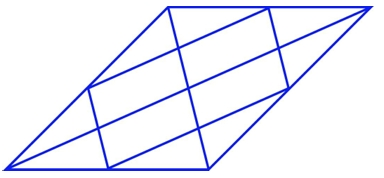
\includegraphics[width=0.5\columnwidth]{figs/img 1.jpeg}
    \caption{}
    \label{fig:placeholder}
\end{figure}


\begin{enumerate}
\begin{multicols}{4}
\item 12
\item 16
\item 20
\item 24
\end{multicols}
\end{enumerate}
\hfill{\brak{\text{GATE ES 2023}}}
\item Students of all the departments of a college who have successfully completed the registration process are eligible to vote in the upcoming college elections. However, by the time the due date for registration was over, it was found that surprisingly none of the students from the Department of Human Sciences had completed the registration process. \\

Based only on the information provided above, which one of the following sets of statement\brak{\text{s}} can be logically inferred with certainty? \\
(i) All those students who would not be eligible to vote in the college elections would certainly belong to the Department of Human Sciences. \\
(ii) None of the students from departments other than Human Sciences failed to complete the registration process within the due time. \\
(iii) All the eligible voters would certainly be students who are not from the Department of Human Sciences. \\

\begin{enumerate}
\begin{multicols}{4}
\item (i) and (ii)
\item (i) and (iii)
\item only (i)
\item only (iii)
\end{multicols}
\end{enumerate}
\hfill{\brak{\text{GATE ES 2023}}}

\newpage

\item Which one of the following options represents the given graph? \\[0.5em]
\begin{figure}[h]
    \centering
    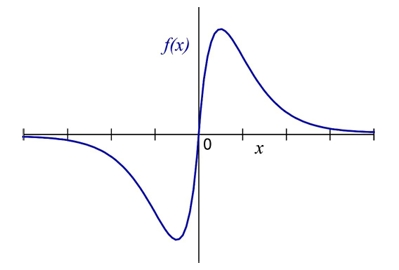
\includegraphics[width=0.5\columnwidth]{figs/img 2.jpeg}
    \caption{}
    \label{fig:placeholder}
\end{figure}


\begin{enumerate}
\begin{multicols}{2}
\item $f(x) = x^2 2^{-|x|}$
\item $f(x) = x \, 2^{-|x|}$
\item $f(x) = |x| \, 2^{-x}$
\item $f(x) = x \, 2^{-x}$
\end{multicols}
\end{enumerate}
\hfill{\brak{\text{GATE ES 2023}}}
\item Which one of the options does NOT describe the passage below or follow from it? \\[0.5em]
We tend to think of cancer as a `modern' illness because its metaphors are so modern. It is a disease of overproduction, of sudden growth, a growth that is unstoppable, tipped into the abyss of no control. Modern cell biology encourages us to imagine the cell as a molecular machine. Cancer is that machine unable to quench its initial command \brak{\text{to grow}} and thus transform into an indestructible, self-propelled automaton. \\[0.5em]
\textit{[Adapted from The Emperor of All Maladies by Siddhartha Mukherjee]} \\[0.5em]

\begin{enumerate}
\item It is a reflection of why cancer seems so modern to most of us.
\item It tells us that modern cell biology uses and promotes metaphors of machinery.
\item Modern cell biology encourages metaphors of machinery, and cancer is often imagined as a machine.
\item Modern cell biology never uses figurative language, such as metaphors, to describe or explain anything.
\end{enumerate}
\hfill{\brak{\text{GATE ES 2023}}}

\newpage

\item The digit in the unit's place of the product $3^{999} \times 7^{1000}$ is \underline{\hspace{1cm}}. 

\begin{enumerate}
\begin{multicols}{4}
\item 7
\item 1
\item 3
\item 9
\end{multicols}
\end{enumerate}
\hfill{\brak{\text{GATE ES 2023}}}
\item A square with sides of length $6 \ \text{cm}$ is given. The boundary of the shaded region is defined by two semi-circles whose diameters are the sides of the square, as shown. The area of the shaded region is \underline{\hspace{1cm}} $\text{cm}^2$. 

\begin{center}
\begin{figure}[h]
    \centering
    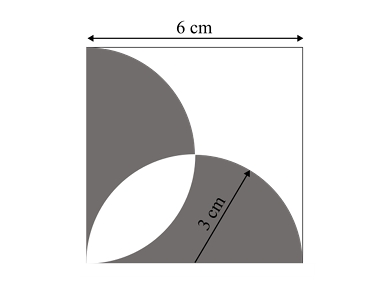
\includegraphics[width=0.5\columnwidth]{figs/img 3.jpeg}
    \caption{}
    \label{fig:placeholder}
\end{figure}

\end{center}

\begin{enumerate}
\begin{multicols}{4}
\item $6\pi$
\item $18$
\item $20$
\item $9\pi$
\end{multicols}
\end{enumerate}
\hfill{\brak{\text{GATE ES 2023}}}

\newpage

\item Given are two ordinary differential equations 
\begin{align}
P: \frac{dy}{dx} + x = x \sin y \\
Q: \frac{dy}{dx} + x y = e^{x} y   
\end{align}
The correct choice is

\begin{enumerate}
\begin{multicols}{2}
\item P is linear; Q is nonlinear
\item P is nonlinear; Q is linear
\item Both P and Q are linear
\item Both P and Q are nonlinear
\end{multicols}
\end{enumerate}
\hfill{\brak{\text{GATE ES 2023}}}

\item $\vec{P}$ and $\vec{Q}$ are square matrices. Consider the following
\begin{align}
X: (\vec{P}^{-1})^{-1} = \vec{P}\\
Y: Symmetric if \vec{Q} = -\vec{Q}^T
\end{align}


The correct choice is

\begin{enumerate}
\begin{multicols}{2}
\item X is TRUE; Y is FALSE
\item X is FALSE; Y is TRUE
\item Both X and Y are TRUE
\item Both X and Y are FALSE
\end{multicols}
\end{enumerate}
\hfill{\brak{\text{GATE ES 2023}}}
\item Given are two infinite series 
\begin{align}
P: \sum \frac{n^2 + 1}{n^2} \\
Q: \sum \left( 1 + \frac{1}{n} \right)^{-n}    
\end{align}


The correct choice is

\begin{enumerate}
\item P is convergent series; Q is divergent series
\item P is divergent series; Q is convergent series
\item Both P and Q are convergent series
\item Both P and Q are divergent series
\end{enumerate}
\hfill{\brak{\text{GATE ES 2023}}}

\item For testing alkalinity for a water sample, first phenolphthalein indicator is added. The water remains colorless. However, when a few drops of methyl orange is added to the sample, the colour turns yellow. As per these observations, the correct choice is

\begin{enumerate}
\item Absence of CO$_3^{2-}$ and/or HCO$_3^-$ but the presence of OH$^-$ ions in the sample
\item Presence of CO$_3^{2-}$ and/or HCO$_3^-$ but the absence of OH$^-$ ions in the sample
\item Absence of CO$_3^{2-}$, HCO$_3^-$ and OH$^-$ ions in the sample
\item Presence of CO$_3^{2-}$, HCO$_3^-$ and OH$^-$ ions in the sample
\end{enumerate}

\newpage

\item Read the following statements

\begin{enumerate}[label=\Roman*.]
\item Photosynthesis takes place within the chloroplasts of the eukaryotes, whereas the breakdown of complex molecules to yield energy takes place in the cytoplasm and in the mitochondria.
\item Photosynthesis takes place within the chloroplasts of the prokaryotes, whereas the breakdown of complex molecules to yield energy takes place in the cytoplasm and in the mitochondria.
\item All living organisms retain the enzymatic machinery to partially oxidise glucose without the help of oxygen. This breakdown of glucose to pyruvic acid is called glycolysis.
\item All living organisms retain the enzymatic machinery to completely oxidise glycerol without the help of oxygen. This breakdown of glycerol to citric acid is called glycolysis.
\end{enumerate}

The correct choice is

\begin{enumerate}
\begin{multicols}{2}
\item I and III are correct
\item II and IV are correct
\item I is correct whereas III is incorrect
\item II is correct whereas IV is incorrect
\end{multicols}
\end{enumerate}
\hfill{\brak{\text{GATE ES 2023}}}
\item Read the following statements

\begin{enumerate}[label=\roman*.]
\item Aerobic heterotrophic bacteria uses organic matter for carbon source and energy source.
\item Aerobic heterotrophic bacteria uses carbon dioxide for carbon source and energy source.
\item Aerobic autotrophic bacteria uses carbon dioxide for carbon source and reduced substances for energy source.
\item Aerobic autotrophic bacteria uses organic matter for getting energy.
\end{enumerate}

The correct choice is

\begin{enumerate}
\begin{multicols}{2}
\item \brak{i} is correct; \brak{iii} is correct
\item \brak{iv} is correct; \brak{i} is incorrect
\item \brak{i} is correct; \brak{iv} is correct
\item \brak{ii} is correct; \brak{iv} is incorrect
\end{multicols}
\end{enumerate}
\hfill{\brak{\text{GATE ES 2023}}}

\item A student wants to decide electron acceptor for aerobic, facultative and anaerobic bacteria. In this context, read the following statements

\begin{enumerate}[label=\roman*.]
\item Dissolved Oxygen \brak{DO} can act as electron acceptor for aerobic bacteria.
\item Nitrite can act as electron acceptor for aerobic bacteria.
\item Dissolved Oxygen \brak{DO} can act as electron acceptor for anaerobic bacteria.
\item Nitrite can act as electron acceptor for facultative bacteria.
\end{enumerate}

The correct choice is

\begin{enumerate}
\item \brak{i} is correct; \brak{iv} is correct
\item \brak{ii} is correct; \brak{iii} is incorrect
\item \brak{i} is correct; \brak{iii} is correct
\item \brak{i} is correct; \brak{ii} is correct
\end{enumerate}
\hfill{\brak{\text{GATE ES 2023}}}

\newpage

\item Which of the following is true according to the Central Pollution Control Board \brak{CPCB}, Government of India's notification issued in the year 2009?

\begin{enumerate}
\item 24 hour averaged standard for PM$_{2.5}$ in ambient air is 60 $\mu$g/m$^3$; 24 hour averaged standard for PM$_{10}$ in ambient air is 100 $\mu$g/m$^3$
\item 24 hour averaged standard for PM$_{2.5}$ in indoor air is 60 $\mu$g/m$^3$; 24 hour averaged standard for PM$_{10}$ in ambient air is 100 $\mu$g/m$^3$
\item 24 hour averaged standard for PM$_{2.5}$ in ambient air is 60 $\mu$g/m$^3$; 24 hour averaged standard for PM$_{10}$ in indoor air is 100 $\mu$g/m$^3$
\item 24 hour averaged standard for PM$_{2.5}$ in indoor air is 60 $\mu$g/m$^3$; 24 hour averaged standard for PM$_{10}$ in indoor air is 100 $\mu$g/m$^3$
\end{enumerate}
\hfill{\brak{\text{GATE ES 2023}}}
\item The sub index values of NO$_2$, SO$_2$ and PM$_{10}$ are 80, 80 and 100, respectively. According to the National Air Quality Index \brak{NAQI} released by the Government of India in the year 2015, the overall NAQI is

\begin{enumerate}
\begin{multicols}{4}
\item 80
\item 260
\item 100
\item 151
\end{multicols}
\end{enumerate}
\hfill{\brak{\text{GATE ES 2023}}}

\item Which of the following is NOT a designated waste category under Bio-medical Waste Management Rules, 2016 of Government of India?

\begin{enumerate}
\begin{multicols}{4}
\item Yellow
\item Green
\item Red
\item Blue
\end{multicols}
\end{enumerate}
\hfill{\brak{\text{GATE ES 2023}}}

\item Consider the following waste categories

\begin{enumerate}[label=\roman*.]
\item Domestic Hazardous Waste
\item Nuclear Waste
\item Sludge from wet scrubbers of hazardous waste treatment processes
\item Chromium bearing residue and sludge from leather tanneries
\end{enumerate}

Which one of the options correctly represents the waste categories NOT covered under Hazardous and Other Wastes \brak{\text{Management and Transboundary Movement}} Rules, 2016 of Government of India?

\begin{enumerate}
\begin{multicols}{2}
\item \brak{i} and \brak{ii} only
\item \brak{i} and \brak{iii} only
\item \brak{ii} and \brak{iv} only
\item \brak{i}, \brak{ii} and \brak{iii} only
\end{multicols}
\end{enumerate}
\hfill{\brak{\text{GATE ES 2023}}}

\newpage

\item Match the following

\begin{center}
\begin{table}[h!]
\centering
\[
\begin{array}{ l l }

\textbf{Plastic Type} & \textbf{Common applications} \\

P. High-density polyethylene (HDPE)   & (i) Garbage bags, bubble packaging \\
Q. Low-density polyethylene (LDPE)    & (ii) Pharmaceutical bottles, Styrofoam cups \\
R. Polyethylene terephthalate (PET)   & (iii) Water bottles \\
S. Polystyrene (PS)                   & (iv) Geomembrane for landfill liner \\

\end{array}
\]
\caption{Plastics and their common applications}
\label{tab:plastics}
\end{table}

\end{center}

\begin{enumerate}
\begin{multicols}{2}
\item P $-$ (iv), Q $-$ (i), R $-$ (iii), S $-$ (ii)
\item P $-$ (i), Q $-$ (iii), R $-$ (ii), S $-$ (iv)
\item P $-$ (iv), Q $-$ (ii), R $-$ (i), S $-$ (iii)
\item P $-$ (ii), Q $-$(iii), R $-$ (iv), S $-$ (i)
\end{multicols}
\end{enumerate}
\hfill{\brak{\text{GATE ES 2023}}}
\item Place the following international conventions/conferences/protocols/declarations 
in the chronological order \brak{\text{oldest to latest}} of their happening

\begin{enumerate}[label=\roman*.]
\item United Nations conference in Stockholm which resulted in the establishment of the United Nations Environmental Program \brak{UNEP}
\item Vienna convention for the protection of the Ozone layer
\item United Nations climate change conference in Glasgow commonly referred as COP26
\item Montreal protocol on phasing out production of substances related to Ozone layer depletion
\end{enumerate}

The correct choice is

\begin{enumerate}
\begin{multicols}{2}
\item i, ii, iv, iii
\item i, ii, iii, iv
\item ii, iv, i, iii
\item iv, iii, ii, i
\end{multicols}
\end{enumerate}
\hfill{\brak{\text{GATE ES 2023}}}

\item The correct ascending order of the following greenhouse gases with respect to their global warming potential relative to CO$_2$ in the time horizon of 100 years is

\begin{enumerate}
\begin{multicols}{2}
\item CH$_4$ $<$ N$_2$O $<$ CFCl$_3$ $<$ CF$_2$Cl$_2$
\item CF$_2$Cl$_2$ $<$ CH$_4$ $<$ N$_2$O $<$ CFCl$_3$
\item CH$_4$ $<$ N$_2$O $<$ CF$_2$Cl$_2$ $<$ CFCl$_3$
\item N$_2$O $<$ CFCl$_3$ $<$ CH$_4$ $<$ CF$_2$Cl$_2$
\end{multicols}
\end{enumerate}
\hfill{\brak{\text{GATE ES 2023}}}

\newpage

\item Read the following statements with reference to the Kyoto Protocol on Climate Change

\begin{enumerate}[label=\roman*.]
\item Each signatory \brak{country} has common and equal responsibility.
\item Clean development mechanism \brak{CDM}, joint implementation \brak{JI} and international emission trading are the three mechanisms under Kyoto Protocol to reduce the greenhouse gas emissions.
\item Under Kyoto Protocol, India has agreed to reduce its greenhouse gas emissions by half by 2050 as compared to 2005 emissions.
\end{enumerate}

Which one of the following is correct choice?

\begin{enumerate}
\begin{multicols}{2}
\item only \brak{i} is TRUE
\item only \brak{ii} is TRUE
\item only \brak{i} and \brak{ii} are TRUE
\item only \brak{ii} and \brak{iii} are TRUE
\end{multicols}
\end{enumerate}
\hfill{\brak{\text{GATE ES 2023}}}
\item Read the following statements

\begin{enumerate}[label=\Roman*.]
\item In environmental laws, the polluter pays principle is enacted to make the polluter responsible for paying for the damage done to the natural environment.
\item The precautionary principle emphasizes caution, pausing and review before going for an innovation that may prove disastrous.
\item The precautionary principle is often used by policy makers in situations where there is the possibility of harm from making a certain decision and conclusive evidence is not yet available.
\end{enumerate}

The correct choice is

\begin{enumerate}
\begin{multicols}{2}
\item I is correct; II and III are incorrect
\item I, II and III are correct
\item I and III are correct; II is incorrect
\item I and II are correct; III is incorrect
\end{multicols}
\end{enumerate}
\hfill{\brak{\text{GATE ES 2023}}}
\item Read the following statements

\begin{enumerate}[label=\Roman*.]
\item The goal of Life Cycle Analysis \brak{LCA} is to assess the environmental impact of products from a system perspective and to identify possible improvement strategies.
\item Environmental Impact Assessment \brak{EIA} is defined as a process of identifying, predicting, and evaluating the likely impacts of a proposed project or development to define mitigation actions to reduce negative impacts and to provide positive contributions to the natural environment and well-being.
\end{enumerate}

The correct choice is

\begin{enumerate}
\begin{multicols}{2}
\item I is correct; II is incorrect
\item II is correct; I is incorrect
\item Both I and II are correct
\item Both I and II are incorrect
\end{multicols}
\end{enumerate}
\hfill{\brak{\text{GATE ES 2023}}}

\newpage

\item For the following major Indian environmental acts
\begin{enumerate}[label=\roman*)]
\item Environmental Protection Act
\item Water Act \brak{\text{Prevention and Control of Pollution}}
\item Air Act \brak{\text{Prevention and Control of Pollution}}
\item The National Green Tribunal Act
\end{enumerate}
the correct chronological order \brak{\text{oldest to latest of their enactment}} is

\begin{enumerate}
\begin{multicols}{2}
\item i, ii, iii, iv
\item ii, i, iii, iv
\item iii, i, iv, ii
\item ii, iii, i, iv
\end{multicols}
\end{enumerate}
\hfill{\brak{\text{GATE ES 2023}}}

\item The kinematic viscosity of glycerin and kerosene are 1.2 times and 0.95 times of that of water, respectively. Glycerin and kerosene flow through two identical porous media having same hydraulic gradient. Assuming Darcy's law is valid for the porous media, the ratio of flow rate of kerosene to that of glycerin is

\begin{enumerate}
\begin{multicols}{2}
\item 1.052
\item 1.140
\item 0.792
\item 1.263
\end{multicols}
\end{enumerate}
\hfill{\brak{\text{GATE ES 2023}}}
\item A researcher compiled the following information about the performance of a kit in an outbreak

\begin{table}[h!]
\centering
\[
\begin{array}{|c|c|c|}
\hline
 & \textbf{Infection state} & \textbf{Kit response} \\
\hline
\text{Disease (probability = 0.002)} & \text{Positive response (probability = 0.98)} &  \\
\text{No Disease} & \text{Positive response (probability = 0.03)} &  \\
\hline
\end{array}
\]
\caption{Probability of kit response under different infection states}
\label{tab:infection}
\end{table}


The probability of detecting an infection for a positive result through the kit would be \_\_\_\_\_\_\_\_\_\_\_\_\_\_\_\_ \brak{\text{rounded off to three decimal places}}.
\hfill{\brak{\text{GATE ES 2023}}}

\item The critical depth in a 2 m wide rectangular channel carrying a discharge of 10 m$^{3}$/s and taking value of acceleration due to gravity ($g$) as 9.81 m/s$^{2}$ is \_\_\_\_\_\_\_\_\_ \brak{\text{in m, rounded off to two decimal places}}.
\hfill{\brak{\text{GATE ES 2023}}}

\item The ratio of the moles of CO$_2$ evolved to the moles of O$_2$ consumed in respiration also called the respiratory quotient, is calculated for a carbohydrate C$_6$H$_{12}$O$_6$ as substrate and found to be 1. Under similar conditions, for a fatty acid C$_{51}$H$_{98}$O$_6$ as substrate, the respiratory quotient is \_\_\_\_\_\_\_\_ \brak{\text{rounded off to two decimal places}}.
\hfill{\brak{\text{GATE ES 2023}}}

\item The value of $\frac{4}{\pi} \int_{0}^{\pi/2} \sin^{2}x \, dx$ is \_\_\_\_\_\_\_\_ \brak{\text{rounded off to two decimal places}}.
\hfill{\brak{\text{GATE ES 2023}}}

\item An S-hydrograph was prepared for a catchment of 240 km$^{2}$ using 3-hour unit hydrograph \brak{\text{1 cm rainfall excess}}. The equilibrium discharge for the S-hydrograph would be \_\_\_\_\_\_\_\_ \brak{\text{in m$^{3}$/s, rounded off to two decimal places}}.
\hfill{\brak{\text{GATE ES 2023}}}

\newpage

\item River water containing two types of spherical suspended particles \brak{\text{clay particles, metal particles}} is retained in a sedimentation tank. The clay particles having diameter of 75 $\mu$m and specific gravity of 2.65 is settling in the tank with a constant velocity. The velocity of clay particles is 2 times of that of metal particles having specific gravity of 8. Assume discrete settling and laminar flow conditions within the sedimentation tank. The estimated diameter of the metal particles is \_\_\_\_\_\_\_\_\_\_\_ (in $\mu$m, rounded off to integer).
\hfill{\brak{\text{GATE ES 2023}}}
\item W1, W2, W3, W9 represent the holding times of 9 water samples, which follow a normal distribution with mean = 8.33 and standard deviation = 4.472. M represents the sample mean value of holding times, which also has a normal distribution. Assuming Z has a standard normal distribution \brak{\text{mean = 0 and standard deviation = 1}}, select the correct statement which describes the expression for calculating the value of type 1 error where

\begin{center}
null hypothesis (H$_0$): \quad M $>$ 6 \\
alternate hypothesis (H$_a$): \quad M $\leq$ 6
\end{center}

\begin{enumerate}
\begin{multicols}{2}
\item P\{Z $<$ (-1.565)\}
\item P\{Z $<$ 1.565\}
\item P\{Z $>$ (-1.565)\}
\item P\{Z $>$ 1.565\}
\end{multicols}
\end{enumerate}
\hfill{\brak{\text{GATE ES 2023}}}
\item Which one of the following statements is NOT correct?
\begin{enumerate}
\item Photophosphorylation is the synthesis of ATP from ADP and inorganic phosphate in the presence of light.
\item The process through which ATP is synthesised by cells \brak{\text{in mitochondria and chloroplasts}} is called phosphorylation.
\item The Calvin cycle \brak{\text{carboxylation, reduction, and regeneration}} occurs in all photosynthetic plants \brak{\text{C3, C4 or any other}}.
\item C3 plants have a special type of leaf anatomy, they tolerate higher temperatures, they show a response to high light intensities, have high rate of photosynthesis and reduced rate of photorespiration as compared to C4 plants.
\end{enumerate}
\hfill{\brak{\text{GATE ES 2023}}}

\newpage

\item Read the following statements
\begin{enumerate}[label=\Roman*.]
\item Bacteriophage is an anaerobic bacterium.
\item Male-specific bacteriophage infect via the pili of other microorganisms including viruses.
\item Bacteriophage is found in human as well as in animal excreta.
\item Bacteriophage can not indicate the presence of bacteria.
\end{enumerate}

The correct choice is
\begin{enumerate}
\begin{multicols}{2}
\item I, III and IV are correct
\item IV is correct; III is incorrect
\item Both III and IV are incorrect
\item Both III and IV are correct
\end{multicols}
\end{enumerate}
\hfill{\brak{\text{GATE ES 2023}}}
\item Read the following statements
\begin{enumerate}[label=\roman*)]
\item In endogenous metabolism by aerobic bacteria, electron acceptor is present inside the cells.
\item In endogenous metabolism by aerobic bacteria, electron acceptor is dissolved oxygen.
\item The endogenous metabolism is linked to fermentative metabolism.
\item In exogenous metabolism by aerobic bacteria, enzyme mediated electron transfer happens within the cells.
\end{enumerate}

The correct choice is
\begin{enumerate}
\begin{multicols}{2}
\item i is correct; iii is correct
\item ii is correct; iii is incorrect
\item iii is incorrect; iv is incorrect
\item iii is correct; iV is correct
\end{multicols}
\end{enumerate}
\hfill{\brak{\text{GATE ES 2023}}}

\item A boiler in an industry, located where high plume rise is expected, releases flue gas with fine particulate matter. Which one of the following options is most suited and efficient if this particulate matter is intended for reuse?
\begin{enumerate}
\item reduce stack height and increase stack diameter
\item use of wet collectors
\item use of flue gas desulfurization (FGD)
\item use of electrostatic precipitator (ESP)
\end{enumerate}
\hfill{\brak{\text{GATE ES 2023}}}

\newpage

\item Match the following

\begin{table}[h!]
\centering
\[
\begin{array}{ll}
\text{J) Dalton's law} & \text{i) Diffusion} \\
\text{K) Fick's law}   & \text{ii) Pressure exerted by a mixture of gases} \\
\text{L) Henry's law}  & \text{iii) Gravitational settling} \\
\text{M) Stoke's law}  & \text{iv) Gas-liquid phase transfer} \\
\end{array}
\]
\caption{Matching of laws with their applications}
\label{tab:laws}
\end{table}

\begin{enumerate}
\begin{multicols}{2}
\item J $-$ ii; K $-$ i; L $-$ iv; M $-$ iii
\item J $-$ iii; K $-$ ii; L $-$ i; M $-$ iv
\item J $-$ ii; K $-$ iii; L $-$ iv; M $-$ i
\item J $-$ i; K $-$ iv; L $-$ ii; M $-$ iii
\end{multicols}
\end{enumerate}
\hfill{\brak{\text{GATE ES 2023}}}
\item Read the following statements

\begin{enumerate}[label=\Roman*.]
\item According to the Liebig's law of minimum, the growth is regulated by the limited factors i.e., resources in scarcity and not by the resources in abundance.
\item Shelford's law of tolerance states that, only the factors present in excess/abundance can affect the growth, development of an organism or rate of biological process.
\item Shelford's law of tolerance states that, an organism's success is based on a complex set of conditions and that each organism has a certain minimum, maximum, and optimum levels of environmental factor or combination of factors that determine success.
\end{enumerate}

The correct choice is

\begin{enumerate}
\item I and II are correct; III is incorrect
\item I and III are correct; II is incorrect
\item II is correct; I and III are incorrect
\item III is correct; I and II are incorrect
\end{enumerate}
\hfill{\brak{\text{GATE ES 2023}}}
\item Read the following statements

\begin{enumerate}[label=\Roman*.]
\item Trivalent chromium has relatively low aqueous solubility, and low mobility in the soil environment. By contrast, hexavalent chromium has a higher aqueous solubility and greater mobility in the soil environment.
\item The chemical reaction between trivalent chromium and zero-valent iron will result in transformed version called hexavalent chromium.
\item Hexavalent chromium is a known carcinogen.
\item Trivalent chromium has relatively higher human toxicity as compared to hexavalent chromium.
\end{enumerate}

The correct choice is

\begin{enumerate}
\item IV is correct; I and III are incorrect
\item II is correct; I and IV are incorrect
\item I and III are correct; II and IV are incorrect
\item I, II and IV are correct; III is incorrect
\end{enumerate}
\hfill{\brak{\text{GATE ES 2023}}}

\newpage

\item Which of the following statements is/are NOT true?

\begin{enumerate}
\item Urban heat island effect in a city can be reduced by increasing trees and vegetation cover in the city.
\item Urban heat island intensity is affected by PM$_{2.5}$ concentrations in a city.
\item Urban heat island intensity increases due to installation of reflective roofs in a city.
\item In comparison with the non-urban areas, urban heat island effect raises night-time temperatures more than daytime temperatures in cities.
\end{enumerate}
\hfill{\brak{\text{GATE ES 2023}}}
\item Read the following statements about aerobic composting of organic fraction of municipal solid waste

\begin{enumerate}[label=\Roman*.]
\item The majority of the odour problem in an aerobic composting process is due to the development of anaerobic conditions within the compost pile.
\item All organic carbon present in the waste will completely biodegrade in 14 days.
\item At high C/N ratio, ammonia would be released and biological activity may also be impeded.
\item Optimum moisture content for aerobic composting process would be 50--60\%. Lower moisture would slow down the biological process. Excessive moisture will make it difficult to maintain aerobic conditions.
\end{enumerate}

The correct choice(s) is/are

\begin{enumerate}
\begin{multicols}{2}
\item I and IV are correct
\item II and III are incorrect
\item I is correct; IV is incorrect
\item II is correct; IV is incorrect
\end{multicols}
\end{enumerate}
\hfill{\brak{\text{GATE ES 2023}}}

\newpage

\item Products P and Q have life cycle phases of material extraction, production, use, and end of life disposal. CH$_4$, CO$_2$ emissions and mass used per functional unit \brak{\text{f.u}}. from the different phases of the products are given in the following tables.

\textbf{Product P}

\begin{table}[h!]
\centering
\[
\begin{array}{|l|c|c|c|}
\hline
\textbf{Phase} & \textbf{CO$_2$ emissions (kg/tonne)} & \textbf{CH$_4$ emissions (kg/tonne)} & \textbf{Mass (tonne/functional unit)} \\
\hline
\text{Material Extraction} & 1.0 & 0.75 & 4.0 \\
\text{Production}          & 1.5 & 1.0  & 2.0 \\
\text{Use}                 & 0.5 & 0.0  & 3.0 \\
\text{End of life disposal}& 1.0 & 0.25 & 1.0 \\
\hline
\end{array}
\]
\caption{Emissions and mass for each life-cycle phase}
\label{tab:emissions}
\end{table}



\vspace{0.3cm}
\textbf{Product Q}

\begin{table}[h!]
\centering
\[
\begin{array}{|l|c|c|c|}
\hline
\textbf{Phase} & \textbf{CO$_2$ emissions (kg/tonne)} & \textbf{CH$_4$ emissions (kg/tonne)} & \textbf{Mass (tonne/functional unit)} \\
\hline
\text{Material Extraction} & 0.75 & 0.75 & 3.0 \\
\text{Production}          & 0.25 & 1.00 & 2.5 \\
\text{Use}                 & 0.00 & 0.50 & 0.75 \\
\text{End of life disposal}& 2.00 & 0.00 & 0.75 \\
\hline
\end{array}
\]
\caption{Emissions and mass for each life-cycle phase}
\label{tab:emissions}
\end{table}


\vspace{0.3cm}
Based upon the information given in the tables and using global warming potential of CH$_4$ equal to 23 kg CO$_2$ per kg of CH$_4$, which of the following statement(s) is/are true?

\begin{enumerate}
\item Greenhouse gas emissions (kg CO$_2$ equivalent/f.u.) from the `Material extraction' phase of product P is higher than that of product Q.
\item Greenhouse gas emissions (kg CO$_2$ equivalent/f.u.) from the `Production' phase of product Q is higher than that of product P.
\item Greenhouse gas emissions (kg CO$_2$ equivalent/f.u.) from the `End of life disposal' is higher for product Q than that of product P.
\item Greenhouse gas emissions (kg CO$_2$ equivalent/f.u.) from the `complete life cycle' of the product P is higher than that of product Q.
\end{enumerate}
\hfill{\brak{\text{GATE ES 2023}}}
\item Second order ordinary differential equation $\frac{d^2 y}{dx^2} - \frac{dy}{dx} - 2y = 0$ has values $y = 2$ and $\frac{dy}{dx} = 1$ at $x = 0$. The value of $y$ at $x = 1$ is \underline{\hspace{2cm}} (rounded off to three decimal places). \hfill{\brak{\text{GATE ES 2023}}}

\item Consider two matrices $\vec{P} = \myvec{ 2 & 3 \\ 1 & 4 }$ and $\vec{Q} = \myvec{ 5 & 4 \\ 0 & 2 }$. If $\vec{R} = (\vec{PQ})^T$ then $\det \vec{R}$ is \underline{\hspace{2cm}} (in integer). \hfill{\brak{\text{GATE ES 2023}}}

\item For the function $f(x) = x\sqrt{4 - x^2}$, the maximum value in the range $-2 \leq x \leq 2$ is \underline{\hspace{2cm}} (rounded off to two decimal places). \hfill{\brak{\text{GATE ES 2023}}}

\item The solubility of gas A is $16\ \text{mg/L}$ in water and its vapor pressure is $0.042\ \text{atm}$ at $25^\circ$C. In a closed system, the gas phase concentration of A is $10^{-3}\ \text{mol/L}$. Assuming ideal gas constant (R) value as $0.0821\ \text{L·atm/mol·K}$, the concentration of gas A in water at $25^\circ$C is \underline{\hspace{2cm}} \brak{\text{in mg/L, rounded off to two decimal places}}. \hfill{\brak{\text{GATE ES 2023}}}

\newpage

\item The following figure \brak{\text{not to the scale}} shows a catchment \brak{\text{Q, S, U, T, Q}} and adjoining rainguage stations P, Q, R, S, U and V. Due to a storm, $20\ \text{mm}$, $25\ \text{mm}$, $30\ \text{mm}$, $15\ \text{mm}$, $22\ \text{mm}$ and $18\ \text{mm}$ rainfall depths were recorded by raingauges at P, Q, R, S, U and V, respectively.
\begin{center}
\begin{figure}[h]
    \centering
    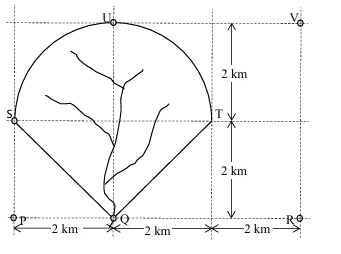
\includegraphics[width=0.5\columnwidth]{figs/img 4.jpeg}
    \caption{}
    \label{fig:placeholder}
\end{figure}
\end{center}

The corresponding mean rainfall over the catchment using Thiessen polygon method is \underline{\hspace{2cm}} \brak{\text{in mm, rounded off to two decimal places}}. \hfill{\brak{\text{GATE ES 2023}}}

\item A trapezoidal canal lined with cement concrete ($n = 0.01$) is designed to carry a discharge of $20\ \text{m}^3/\text{s}$ at a bed slope $1$ in $400$. If the bed width is twice the depth of flow and side slope of the canal section is $2$ (1 vertical: 2 horizontal) then the corresponding depth of flow will be \underline{\hspace{2cm}} \brak{\text{in m, rounded off to two decimal places}}. \hfill{\brak{\text{GATE ES 2023}}}

\newpage

\item A plunger weighing $314\ \text{kN}$ is balanced in a cylindrical vessel of diameter $1.5\ \text{m}$ and filled with an oil \brak{\text{specific gravity $0.9$}} as shown in the following figure \brak{\text{not to the scale}}.

\begin{center}
\begin{figure}[h]
    \centering
    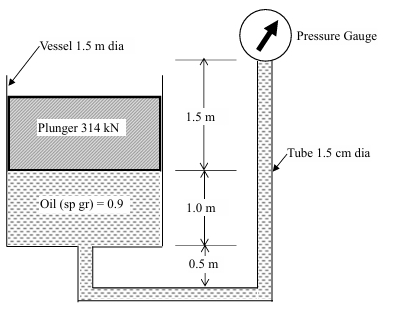
\includegraphics[width=0.5\columnwidth]{figs/img 5 (2).jpeg}
    \caption{}
    \label{fig:placeholder}
\end{figure}

\end{center}

If a pressure gauge is connected with the vessel using $1.5\ \text{cm}$ diameter tube, the reading of the gauge will be \underline{\hspace{2cm}} \brak{\text{in kPa, rounded off to two decimal places}}. \hfill{\brak{\text{GATE ES 2023}}}

\item A fully penetrating well is installed in a homogenous and isotropic confined aquifer. The aquifer has uniform thickness of $16\ \text{m}$ and hydraulic conductivity of $25\ \text{m/d}$. Water is being pumped out from the well at a constant rate of $0.1\ \text{m}^3/\text{s}$ till steady state condition is reached. If a drawdown of $3.5\ \text{m}$ is observed at a distance of $75\ \text{m}$ from the well then the drawdown at a distance of $150\ \text{m}$ from the well will be \underline{\hspace{2cm}} \brak{text{in m, rounded off to two decimal places}}. \hfill{\brak{\text{GATE ES 2023}}}

\newpage

\item A biological reactor is getting wastewater containing 1 mole/L acetate ions as carbon source. The following reaction takes place in the bio-reactor:
\[
0.125\mathrm{CH_3COO^-} + 0.0295\mathrm{NH_4^+} + 0.103\mathrm{O_2} \rightarrow 0.0295\mathrm{C_5H_7O_2N} + 0.0955\mathrm{H_2O} + 0.095\mathrm{HCO_3^-} + 0.007\mathrm{CO_2}
\]
Assume that all acetate ions are consumed and ammonia serves as a nutrient source. Given that 1 g acetate exerts 1.07 g COD; 1 mole bacteria = 113 g VSS; 1 mole acetate ion = 59 g. Value of observed yield is \underline{\hspace{2cm}} \brak{\text{in g VSS/g COD, \textit{rounded off to two decimal places}}}.  
\hfill{\brak{\text{GATE ES 2023}}}

\item A flask \brak{\text{100 mL volume}} has wastewater, which has 0.12 mg/L geosmin. Activated carbon is added in this flask for adsorbing geosmin as per the Freundlich isotherm model ($Q = 2.6C^{0.73}$ where $Q$ is mg adsorbate/mg adsorbent and $C$ is the equilibrium concentration in mg/L). Activated carbon to be added in this flask for getting final remaining geosmin concentration of 0.05 mg/L would be \underline{\hspace{2cm}} \brak{\text{in mg/L, \textit{rounded off to three decimal places}}}.  
\hfill{\brak{\text{GATE ES 2023}}}

\item A pipeline is designed to deliver 20 L/s of an oil \brak{\text{kinematic viscosity = $6\times 10^{-6}$ m$^2$/s and specific gravity = 0.9}} under the laminar flow condition. The minimum diameter of the pipe will be \underline{\hspace{2cm}} \brak{\text{in m, \textit{rounded off to two decimal places}}}.  
\hfill{\brak{\text{GATE ES 2023}}}

\item You are doing an experiment to find out BOD$_5$ of a wastewater. You have taken 25 mL wastewater having ultimate BOD of 75 mg/L and placed it into 300 mL BOD bottle and filled it with dilution water. The initial DO of the diluted sample is 6.5 mg/L. On the 5\textsuperscript{th} day, you were not able to measure the DO due to unavoidable circumstances. However, the DO at the end of the 7\textsuperscript{th} day is found to be 1.25 mg/L. Assume all the experiments are done at the same temperature, and no biodegradable organics are present in the dilution water. The BOD$_5$ of the wastewater sample is \underline{\hspace{2cm}} \brak{\text{in mg/L, \textit{rounded off to two decimal places}}}.  
\hfill{\brak{\text{GATE ES 2023}}}
\item In a 30 m$^3$ room, a stove in operation consumes wood at the rate of 0.25 kg/h. The inflow and outflow rate of air in the room is the same, i.e., 500 m$^3$/h. This stove emits a VOC species at a rate of 0.2 g/kg-wood. The VOC species gets converted to CO$_2$ at a rate of 0.4 per hour. Given: (i) the air in the room is completely mixed, (ii) initial concentration of the VOC species in the room is negligible, and (iii) concentration of the VOC species in the air entering the room is negligible. The concentration of the VOC species due to two hours of stove operation in the room is \underline{\hspace{2cm}} \brak{\text{in $\mu$g/m$^3$, \textit{rounded off to one decimal place}}}.  
\hfill{\brak{\text{GATE ES 2023}}}

\item A city generates on average 1000 metric tonnes/day of municipal solid waste and follows integrated waste management system. 15\% of the total waste is recycled, 40\% of the total waste is used to produce compost, 25\% of the total waste is converted to refuse derived fuel \brak{RDF} with 80\% efficiency. Remaining is disposed of in a sanitary landfill. The calorific value of the RDF is 15 MJ/kg, which is further used to generate electricity. The electrical energy that could be generated from the RDF with a thermal to electrical energy conversion efficiency of 20\% is \underline{\hspace{2cm}} \brak{\text{in MWh/d, \textit{rounded off to two decimal places}}}.  
\hfill{\brak{\text{GATE ES 2023}}}

\newpage

\item An industry with an effective stack height of 80 m emits 1200 g/h of CO. The windrose plotted using the meteorological data at the top of the stack, and the relation between dispersion coefficients and wind direction are given below:

\begin{center}
\begin{figure}[h]
    \centering
    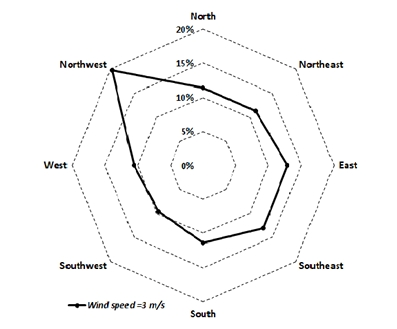
\includegraphics[width=0.5\columnwidth]{figs/img 6 (2).jpeg}
    \caption{}
    \label{fig:placeholder}
\end{figure}

\end{center}

\begin{table}[h!]
\centering
\[
\begin{array}{|c|c|c|}
\hline
\textbf{Wind Direction} & \textbf{Crosswind direction (m)} & \textbf{Vertical direction (m)} \\
\hline
\text{Northeast} & 50 & 20 \\
\text{North}     & 45 & 30 \\
\text{Northwest} & 40 & 35 \\
\text{East}      & 45 & 30 \\
\text{Southeast} & 55 & 35 \\
\text{South}     & 60 & 40 \\
\text{Southwest} & 65 & 45 \\
\text{West}      & 70 & 50 \\
\hline
\end{array}
\]
\caption{Crosswind and vertical directions for different wind directions}
\label{tab:wind}
\end{table}


During the maximum duration of the year, the ground level PM$_{2.5}$ concentration at the downwind distance of 2 km \brak{\text{at the plume centerline}} from the stack is \underline{\hspace{2cm}} \brak{\text{in $\mu$g/m$^3$, \textit{rounded off to two decimal places}}}.  
\hfill{\brak{\text{GATE ES 2023}}}

\newpage

\item Ms. Anita uses a BS-IV two wheeler petrol scooter, with a mileage of 50 km/L, to travel 30 km every day. She exchanges this two wheeler with an electric scooter, which consumes electricity at 0.1 kWh/10 km. Assuming the cost of petrol and electricity are fixed at Rs. 90 per L and Rs. 3.5 per kWh, respectively, and maintenance cost of both BS-IV two wheeler and electric scooter is negligible, the operational cost saved in a year by Ms. Anita is \underline{\hspace{2cm}} \brak{\text{in Rs., in integer}}.  
\hfill{\brak{\text{GATE ES 2023}}}

\item Ultimate analysis of a municipal solid waste sample is given below:

\begin{table}[h!]
\centering
\[
\begin{array}{|c|c|}
\hline
\textbf{Percent by weight} & \textbf{Value (\%)} \\ \hline
\text{Carbon}    & 48 \\
\text{Hydrogen}  & 6  \\
\text{Oxygen}    & 35 \\
\text{Nitrogen}  & 6  \\
\text{Ash}       & 5  \\ \hline
\end{array}
\]
\caption{Elemental composition by weight}
\label{tab:composition}
\end{table}

For 1 kg of the municipal solid waste burnt, assuming that air contains only nitrogen and oxygen, maximum CO$_2$ emitted is \underline{\hspace{2cm}} \brak{\text{in kg, \textit{rounded off to three decimal places}}}.  
\hfill{\brak{\text{GATE ES 2023}}}

\item An adult of 65 kg weight and life span of 65 years drinks water for 5 years, which is contaminated with toluene of concentration 0.15 mg/L. For toluene, reference dose is 0.200 mg/kg$\cdot$d. The person drinks 2 L of water per day. The hazard quotient from the toluene exposure for the adult will be \underline{\hspace{2cm}} \ brak{\text{\textit{rounded off to three decimal places}}}.  
\hfill{\brak{\text{GATE ES 2023}}}

\item An aeration tank needs to be installed for the removal of VOC from water, where the required rate of flow of water through the aeration tank is 180,000 m$^3$/d. Permissible limit of VOC in the water is 12 $\mu$g/L. The saturation concentration of VOC is 5 $\mu$g/L and gas transfer rate constant is 0.40 per second at 25$^\circ$C. The initial concentration of VOC in the water is 33 $\mu$g/L. The volume of the aeration tank to satisfy the permissible limit of VOC at 25$^\circ$C is \underline{\hspace{2cm}} \brak{\text{in m$^3$, \textit{rounded off to two decimal places}}}.  
\hfill{\brak{\text{GATE ES 2023}}}
\end{enumerate}
\centering
$\varmathbb{END OF QUESTION PAPER}$
\end{document}